\documentclass[12pt]{article}
\usepackage{graphicx}
\usepackage{amsmath}
\begin{center}
\textbf{Manish Milind Tathode}
\end{center}
\hline
\label{sec:ManishMilindTathode}
\begin{document}
\begin{flushleft}
Flat no:9,Sai-Srusht apartment,\hspace{1in}Contact:9970169658\\ 
Frank Pinto colony\hspace{1in} Email Id:manishtathode@gmail.com\\
Jail Road, Nasik Road \\ 
Nasik-422101\\Maharashtra.
\vspace{-4ex}
\begin{figure}[h]
\begin{flushright}
		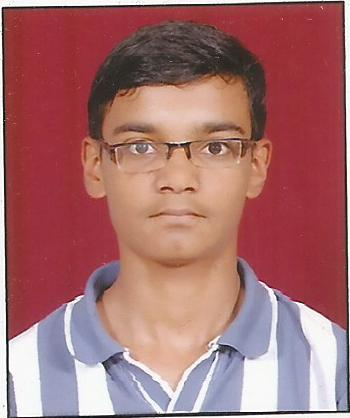
\includegraphics[width=0.2\linewidth,angle=+0]{C:\Users\Manish PC\Desktop\manish_resume\manish_resume.jpg}
	\label{fig:IMG-20160525-WA0000}
	\end{flushright}
\end{figure}
\vspace{-4ex}
\begin{flushleft}
\textbf{OBJECTIVE}: To serve the society by serving organisational goals with increasing efforts and excellence in the field of technology. }
\end{flushleft}
\begin{flushleft}
\caption{\textbf{EDUCATION:}}\vspace{2ex}
\begin{tabular}{|l|c|c|c|c|r|}  \hline
Degree & College/School & University & Passing Year &  Percentage\\ \hline
B.Tech & Walchand COE, & Shivaji & 2017 & 8.5\\ 
Electrical & Sangli & University & & (CPI) \\ \hline
\end{tabular}
\end{flushleft}

\begin{flushleft}
\textbf{PROJECTS:}
\end{flushleft}
\begin{enumerate}
\item Multiple electrical parameter measurement & protective alarming unit under guidance of Dr. A. P. Vaidya
\item  Automatic lighting control using instrumentation amplifier.
\item Image processing based autonomous robot using camera for eYRC+. 
\end{enumerate}
\begin{flushleft}
\textbf{TRAINING AND INTERNSHIP :}
\begin{itemize}
\item Industrial Training at �Traction Machine Workshop, Nashik�, from 16th July 2015
to 25th July 2015.
\item Industrial Training at �Thermal Power station, Eklahare , Nasik� in June 2015.
\end{itemize}
\end{flushleft}
\begin{flushleft}
\textbf{RESEARCH AND PUBLICATIONS:}\\
1.
\end{flushleft}
